\documentclass[a4paper]{book}

% Preambulo por defecto
% Paquetes para usar bien el idioma español
\usepackage[spanish,es-tabla]{babel}
\selectlanguage{spanish}
\usepackage[utf8]{inputenc}

% Paquetes para usar mejores imagenes
\usepackage{graphicx}

% Paquetes para links y tabla de contenidos en el PDF
\usepackage{hyperref}
\hypersetup{colorlinks=true,allcolors=blue}
%\usepackage{hypcap}

% Paquetes para mejores tablas
\usepackage{booktabs}

% Mejor matematica
\usepackage{amsmath}

% Fuentes de las imagenes
\usepackage[absolute,overlay]{textpos}

% Paquete captions
\usepackage[justification=centering,labelformat=empty,labelsep=none]{caption}

% Opciones para ticks
\usepackage{tikz}
\usetikzlibrary{shapes,arrows,positioning}

\tikzstyle{decision} = [diamond, draw, fill=blue!20, text width=4em, text badly centered, node distance=2cm, inner sep=0pt,on grid]
\tikzstyle{block} = [rectangle, draw, fill=blue!20, text width=8em, text centered, rounded corners, minimum height=2em,on grid]
\tikzstyle{line} = [draw, -latex]

% Citas bibliograficas
\usepackage[backend=biber]{biblatex}
\renewcommand{\footnotesize}{\tiny}
\addbibresource{biblio.bib}

% Mejoro las captions
\setbeamertemplate{caption}{\raggedright\insertcaption\par}

\setbeamertemplate{caption}{%
\begin{beamercolorbox}[wd=0.85\paperwidth, sep=.2ex]{block body}\insertcaption%
\end{beamercolorbox}%
}


% Sacar barra de navegacion
\setbeamertemplate{navigation symbols}{}%remove navigation symbols

% Transparencias en items
\setbeamercovered{transparent}

% Estilo de diapositivas
% \usetheme{Boadilla}
\usecolortheme{whale}
\usecolortheme{orchid}

\usepackage{fancyvrb}
% Ejemplos, observaciones y teorema
\theoremstyle{definition}
\newtheorem{exa}{Ejemplo}[section]
\newtheorem{obs}{Observación}[section]
\newtheorem{act}{Actividad}[section]


% Referencias menu
\newtoggle{FirstOne}%
\newcommand*{\menu}[1]{%
\toggletrue{FirstOne}%
\foreach \x in {#1} {%
\iftoggle{FirstOne}{}{${}\rightarrow{}$}
\emph{\x}%
\global\togglefalse{FirstOne}%
}%
}%

% Referencias archivo
\newtoggle{SecondOne}%
\newcommand*{\file}[1]{%
\toggletrue{SecondOne}%
\foreach \x in {#1} {%
\iftoggle{SecondOne}{}{${}/{}$}%
\texttt{\x}%
\global\togglefalse{SecondOne}%
}%
}%

\usepackage{emptypage}


\title{{Nivel 2: Herramientas de teledetecci\'on cuantitativa}\\
\emph{Gu\'{\i}a de actividades: Uso del suelo en el departamento de Iguaz\'u,
provincia de Misiones}}
\date{2017-1}
\author{Francisco Nemiña\thanks{\texttt{fnemina@conae.gov.ar}}}
\affil{Unidad de Educacion y Formacion Masiva \\ Comisi\'on Nacional de Actividades Espaciales}

\graphicspath{{./figs/}}



\begin{document}
\frontmatter
\maketitle

\tableofcontents
\mainmatter
\chapter*{Introducción}

\label{sec:intro}

La utilización de imágenes satelitales permite analizar grandes extensiones del
territorio, contando con un registro histórico con el cual realizar
comparaciones.

En la provincia de Misiones, el departamento de Iguaz\'u es lindante a Brasil y
Paraguay siendo parte de la zona conocida como triple frontera
perteneciente a la ecorregi\'on conocida como \emph{selva paranaense} (Figura \ref{parque}). Dentro
del mismo podemos encontrar la Represa de Urugua-\'{\i} y el Parque Nacional
Iguaz\'u. El departamento tiene un area de $2.736 km^2$ y una poblaci\'on de
$82.227$ seg\'un el \'u;timo senso del INDEC.

\begin{figure}[h!]
  \centering
  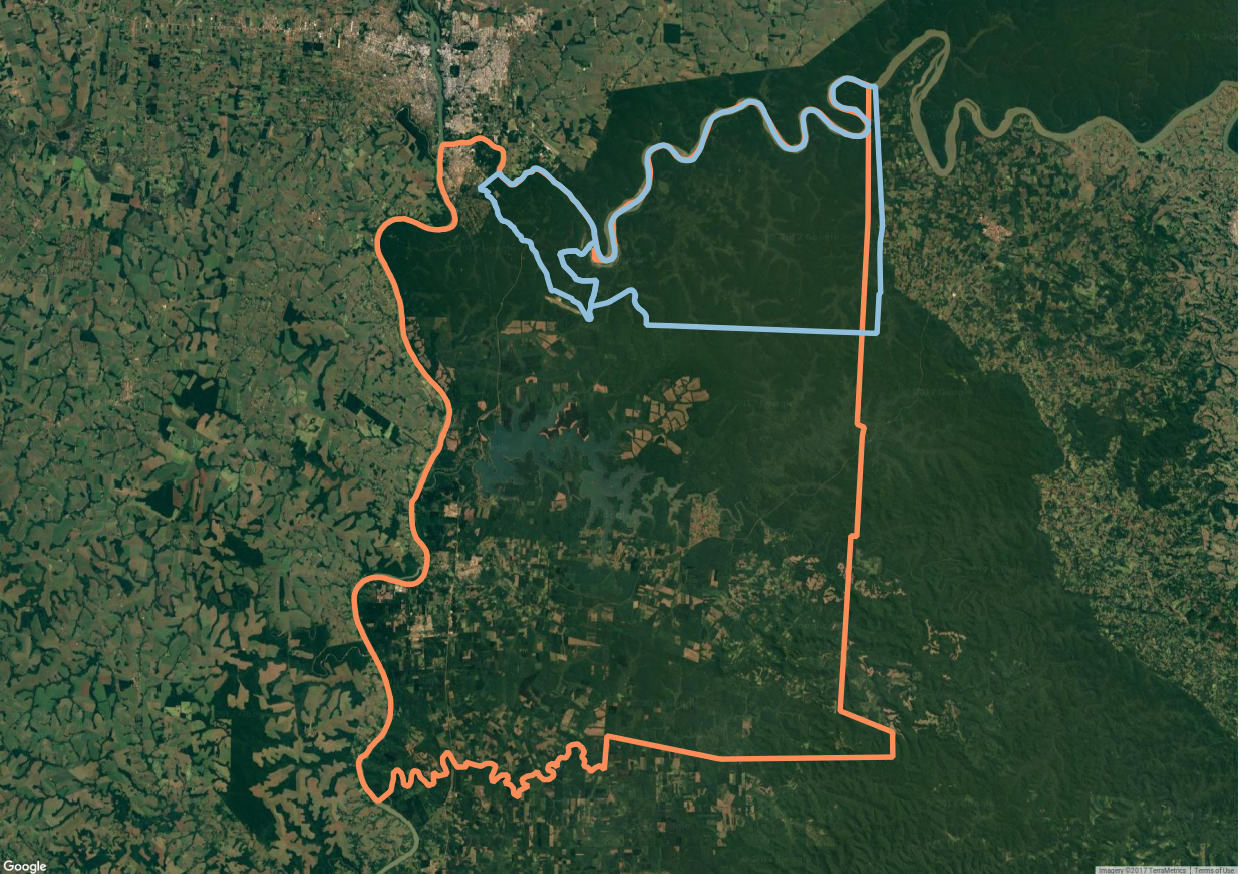
\includegraphics[width=0.8\textwidth]{triple.png}
  \caption{Departamento de Iguaz\'u, en rosa, y parque natural Iguaz\'u, en celeste.}
  \label{parque}
\end{figure}

Tomaremos entonces al departamento como \'area de estudio durante este curso
con el objetivo de obtener un mapa de uso y cobertura dentro del mismo que nos
permita estimar y validar  las \'areas correspondients a los mismos.

Utilizaremos para esto imagenes satelitales de los satelites Landsat 8, Landsat 7 y
el producto de MOD13Q1 obtenido de los satelites TERRA y AQUA obtenidas durante
el periodo 2000-2016.

\section{Organizacion del curso}

El curso se divide en dos partes. En la primera trabajaremos con la compresion
del espacio espectral y el uso de las imagenes satelitales para extraer valores
continuos de las variables biofisicas.

En el capitulo \ref{viaje}, \nameref{viaje}, estudiaremos la firma espectral de
distintas coberturas, veremos como se relacionan con las propiedades biofisicas
de ellas y por ultimo introduciremos el concepto de espacio espectral como el
lugar natural donde realizar el analisis en teledeteccion.

En el capitulo \ref{rebotando}, \nameref{rebotando}, estudiaremos distintas
formas de obtener la reflectancia de las coberturas a partir de los datos obtenidos
por un satelite. En el estudiaremos metodos de correccion atmosferica basados
en propiedades estadisticas de las imagenes y en el modelado de la atmosfera.

En el capitulo \ref{abaco}, \nameref{abaco}, veremos como a partir de los valores
de reflectancia para una cobertura y operaciones matematicas entre los mismos,
podemos obtener los valores de variables biofisicas continuass como pueden ser
el contenido de clorofila o humedad.

En la segunda parte del curso vamos a trabajar mas en detalle con el espacio
espectral y vamos a usar sus propiedades para extraer informacion categorica de
las imagenes.

En el capitulo \ref{rotaciones}, \nameref{rotaciones}, veremos como utilizar
herramientas geometricas en el espacio de reflectancias para resaltar distintas
propiedades de las imagenes y poner en evidencia cuales son las zonas del espectro
que mas informacion aportan sobre nuesta zona de interes. Comenzaremos en este
capitulo tambien a analizar el contexto temporal para nuestras imagenes.

En el capitulo \ref{otrolado}, \nameref{otrolado}, veremos como utilizar herramientas
que no requieren de conocimiento previo del area de estudio para realizar segmentaciones
en el espacio de fases de la imagen, que luego podremos utilizar para obtener mapas
de uso y cobertura. Comenzaremos en este capitulo tambiena analizar el contexto
espacial de cada pixel.

En el capitulo \ref{educando}, \nameref{educando}, veremos otros metodos para extraer
informacion categorica sobre las imagenes satelitales al estudiar distintas
formas de clasificacion supervisada. Comenzaremos en este capitulo tambien a
analizar mas en detalle cuales son las coberturas que mayores problemas generan al
momento de realizar clasificaciones

En el capitulo \ref{pos}, \nameref{pos}, veremos algunas tecnicas de postprocesamiento
que nos permitiran analizar el contexto espacial de nuestras clasificaciones y
comenzar a calcular areas de cobertura para nuestras imagenes con su correspondiente incerteza.

\subsection{Cronograma}

Duranto el curso trabajaremos con el siguiente cronograma

\begin{itemize}
  \item[25/4] Instalar el QGIS y el R. Ver apendice.
  \item[26/4] \nameref{viaje}
  \begin{itemize}
    \item Clase teorica: radiancia y reflectancia. Firmas espectrales y espacio espectral.
    \item Clase practica: capitulo \ref{viaje} de la guida practica.
    \item Lectura recomendada: Remote sensing digital Image Analysis - Jogn A. Richards. Capitulos 1 y 3
  \end{itemize}
  \item[2/5] Entrega del cuestionario 1.
  \item[3/5] \nameref{rebotando}
  \begin{itemize}
    \item Clase teorica: Transferencia radiativa. Metodos estadisticos y modelado de la atmosfera.
    \item Clase practica: capitulo de \ref{rebotando} la guia practica.
    \item Lectura recomendada: Remote sensing digital Image Analysis - Jogn A. Richards. Capitulos 2
  \end{itemize}
  \item[9/5] Entrega del cuestionario 2.
  \item[10/5] \nameref{abaco}
  \begin{itemize}
    \item Clase teorica: C\'alculo de indices espectrales
    \item Clase practica: capitulo de \ref{abaco} la guia practica.
    \item Lectura recomendada: Quantitative Remote Sensing - ShunLin Liang. Capitulos 8
  \end{itemize}
  \item[16/5] Entrega del cuestionario 3.
  \item[17/5] Clase de consulta.
  \item[23/5] Entrega del trabajo practico 1.
  \item[24/5] \nameref{rotaciones}
  \begin{itemize}
    \item Clase teorica: Transformada Tasseled Cap y Analisis por componentes principales.
    \item Clase practica: capitulo de \ref{rotaciones} la guia practica.
    \item Lectura recomendada: Remote sensing digital Image Analysis - Jogn A. Richards. Capitulos 6
  \end{itemize}
  \item[30/5] Entrega del cuestionario 4.
  \item[31/5] \nameref{otrolado}
  \begin{itemize}
    \item Clase teorica: Metodos de clasificacion no supervisados.
    \item Clase practica: capitulo de \ref{otrolado} la guia practica.
    \item Lectura recomendada: Remote sensing digital Image Analysis - Jogn A. Richards. Capitulos 9
  \end{itemize}
  \item[6/6] Entrega del cuestionario 5.
  \item[7/6] \nameref{educando}
  \begin{itemize}
    \item Clase teorica: Metodos de clasificacion supervisados.
    \item Clase practica: capitulo de \ref{educando} la guia practica.
    \item Lectura recomendada: Remote sensing digital Image Analysis - Jogn A. Richards. Capitulos 8
  \end{itemize}
  \item[13/6] Entrega del cuestionario 6.
  \item[14/6] \nameref{pos}
  \begin{itemize}
    \item Clase teorica: Tecnicas post clasificacion.
    \item Clase practica: capitulo de \ref{pos} la guia practica.
    \item Lectura recomendada: Making better use of accuracy data in land change studies: Estimating accuracy and
area and quantifying uncertainty using stratified estimation - Olofsson et al.
  \end{itemize}
  \item[20/6] Entrega del cuestionario 7.
  \item[21/6] Clase de consulta. Arreglar horario.
  \item[27/6] Entrega del trabajo practico 2.
  \item[30/6] Entrega de certificados.
\end{itemize}

\subsection{Forma de aprobacion}
Para aprobar el curso se deben juntar al menos 100 puntos entre las distintas actividades.
Adem\'as se deber\'a completar un cuestionario \emph{obligatorio} sobre el curso
al finalizar el mismo.

La nota final del curso estara dada por la siguiente

\begin{itemize}
\item 0 - 99 - No aprobó
\item 100-109 - Seis
\item 110-129 - Siete
\item 130-169 - Ocho
\item 170-189 - Nueve
\item 190-200 - Diez
\end{itemize}

para obtener puntos puede realizarse de la siguiente manera

\begin{itemize}
  \item Cada cuestionario: 0 a 10 puntos. Máximo 70.
  \item Cada tarea: 0 a 50 puntos. Máximo 100.
  \item Participar en la plataforma: 0 a 10 puntos. Sin máximo.
\end{itemize}

\section{Materiales del curso}
Todos los materiales del curso, con sus correspondientes editables, pueden
encontrarse en el repositorio de github \url{https://github.com/fnemina/curso-sopi-herramientas-cuantitativas}.

En caso de encontrar cualquier problema en los materiales puede reportarlo ahi y sera
subsanado en el menor tiempo posible.

\part{Variables continuas}

\chapter{Un viaje del sol a los p\'ixeles.}
\label{viaje}
En esta primera práctica nos familiarizaremos con las interfaces gráficas del
qgis y de R-studio. Para esto comenzaremos a analizar la imagen correspondiente
a la zona de estudio del año 2015 desde el punto de vista espectral. Son
nuestros objetivos

\begin{itemize}
    \item Poder cargar una imagen en qgis.
    \item Digitalizar coberturas en qgis.
    \item Poder cargar un archivo raster y uno vectorial en R.
    \item Realizar un análisis estadistico de la imagen como un todo y de las
        distintan coberturas digitalizar en R.
\end{itemize}
\subsection{Exploración de imagenes con el qgis}

Comenzamos abriendo la imagen \file{LC82240782016304LGN00.vrt} que se encuentra
en la carpeta \file{raster\_data,LC82240782016304}. Esta image  corresponde al 
departamento de Iguazu en la provincia de corriente. La misma fue obtenida por 
el satelite Landsat 8 durante el mes de noviembre de 2016.
 
Para esto vamos al menú \menu{Capa, Añadir capa, Añadir capa ráster}. Navegamos 
hasta la carpeta \file{raster\_data/LC8224078201630} y abrimos el archivo
\file{LC82240782016304LGN00.vrt}. Una vez abierto el mismo podremos encontrarlo
en el \menu{Panel de capas} de q-gis donde podremos manejar la visualización del
mismo y estudiar las propiedades de dicha capa.

\begin{figure}[htb]
\begin{center}
    
\includegraphics[scale=0.2]{move.png}
\end{center}
\caption{Herramientas para moverse dentro de la imagen. De izquierda a derecha:
    1. Desplazar mapa, 2. Desplazar mapa a la seleccion, 3. Acercar zum, 4.
    Alejar zum, 5. Zum a la resolucion nativa, 6. Zum general, 7. Zum a la
    seleccion, 8. Zum a la capa, 9. Zum anterior, 10. Zum siguiente, 11.
    Actualizar.}
\label{fig:move}
\end{figure}

Para realizar cambiar la visualizacion y explorar los datos de una capa, hacemos
click derecho sobre la misma y luego seleccionamos la opciopn
\menu{Propiedades}. Dentro de las propiedades de la capa podemos ir a la pestaña
\menu{General} para ver datos como el nombre de la capta\footnote{Es un buen
momento para ponerle uno mas sencillo}, la cantidad de filas y columnas del
archivo, el valro digital no valido, el sistema de referencias de coordenadas
entro otros. 

\begin{figure}[htb]
\begin{center}
    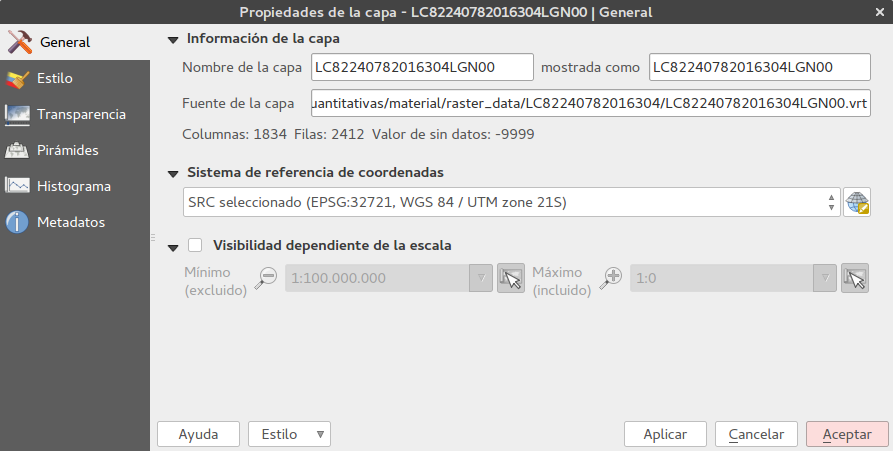
\includegraphics[scale=0.2]{general.png}
\end{center}
\caption{Pestaña general de propiedades de una capa. En la misma se pueden ver
    los datos mas importantes sobre la misma como la cantidad de filas y
    columnass, el nombre y el sistema de referencia de coordenadas.}
\label{fig:general}
\end{figure}

Podemos ir luego a la pestaña de estilo para cambiar la visualizacion de la
imagen. En la misma podemos elegir de que color mostraremos cada una de las
capas ademas de elegir el tipo de realce que deseamos aplicar. Es importante
remarcar en este caso que una vez elegidas las badnas debemos hacer click en el
boton \menu{Cargar} para seleccionar los valores maximos y minimos de las
bandas para el realcec.

\begin{figure}[htb]
\begin{center}
    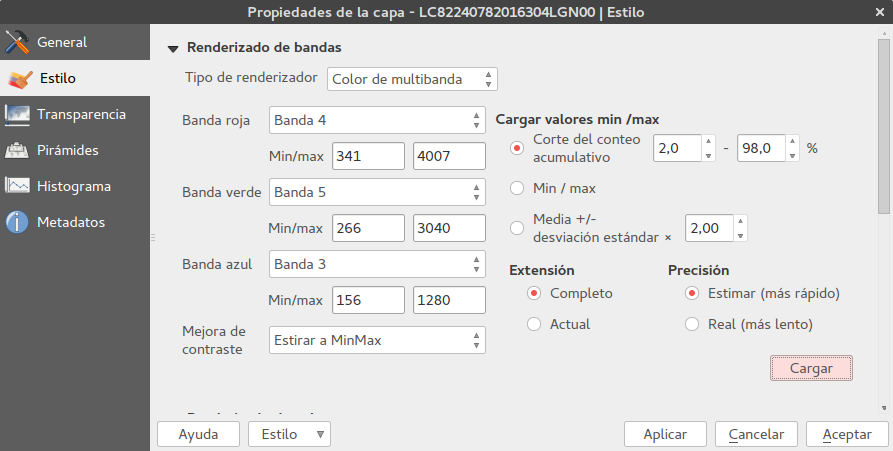
\includegraphics[scale=0.2]{estilo.png}
\end{center}
\caption{Estilos de visualizacion de una capa raster. Los estilos posibles son:
    1. Color de multibanda, 2. En paleta, 3. Unibanda gris, 4. Unibanda
    pseudocolor. Puede explorar cada uno por separado ya que todos tendran
    distintas utilidades.}
\label{fig:estilo}
\end{figure}

\begin{act} 
    Cambie la combinación de bandas de la imagen L8 y muévase  dentro de la
    misma. Identifique zonas de coberturas uniformes. Pruebe cambiar de
    combinacion de bandas y decida si dichas zonas siguen siendo uniformes luego
    del cambio.
\end{act}

\begin{act}
    Encuentre el sistema de coordenadas en el cual se encuentra la imagen.
\end{act}

Para identificar la informacion correspondiente a un punto en el espacio podemos
utilizar la herramienta \menu{Identificar un objeto espacial}. Al habilitarla y
hacer click sobre un punto de la imagen veremos datos de la misma como por
ejemplo los valores de reflectancia del pixel seleccionado. Dichos valores
pueden mostrarse como Arbol, Tabla o Grafo segun como sea mass comodo.

\begin{figure}[htb]
\begin{center}
    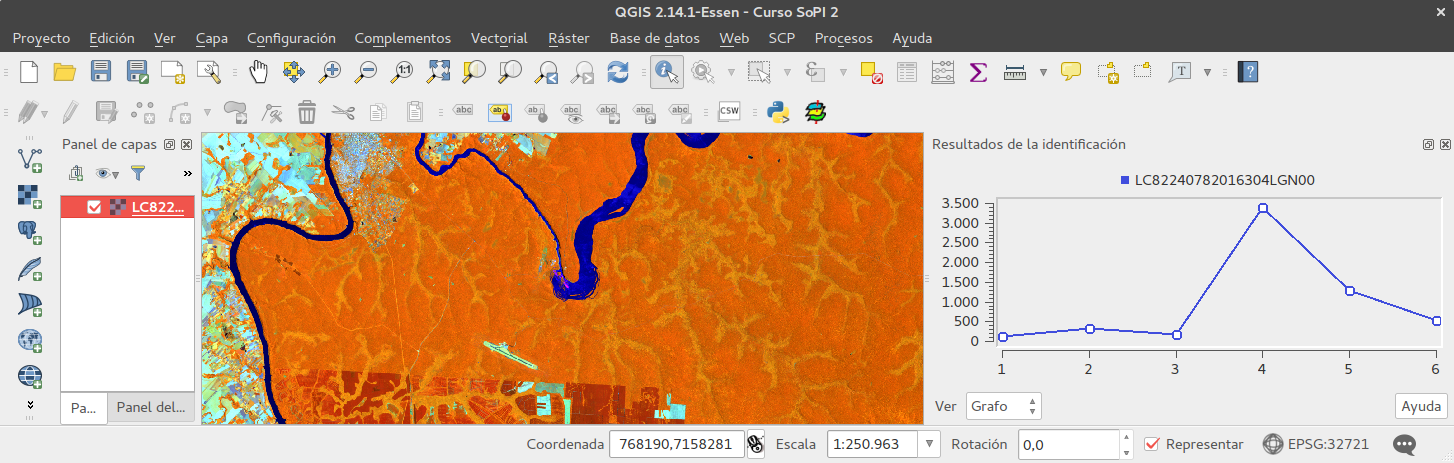
\includegraphics[scale=0.2]{grafo.png}
\end{center}
\caption{Identificacion de un pixel correspondiente a la selva paranaense
    mostrada como grafo. }
\label{fig:grafo}
\end{figure}

\begin{act}
   Utilizando la herramienta identificar objetos espaciales encuentre los
   valores de reflectancia de distintas coberturas. Grafique estos  valores en
   una firma espectral y en el espacio de fases nirrojo.
\end{act}

\subsection{Creacion de capas vectoriales}

Veamos ahora como crear capas vectoriales con las cuales podamos extraer
informacion sobre nuestra zona.

Con la herramienta nueva capa de archivo shape es posible digitalizar zonas de
la imagen para su posterior analisis. Para esto puede hacer click en el boton
del panel lateral. Podemos agregar los campos que sean necesarios para nuestra
capa vectorial en este momento. Crearemos al menos los campos MC\_ID como entero
de longitud 1 y Comment como texto de 80 caracteres. Guardela en la carpeta 
\file{vector\_data/} con el nombre \file{firmas.shp}. Recuerde elegir el sistema 
de coordenadas correspondiente a la imagen anterior. 

\begin{figure}
\begin{center}
    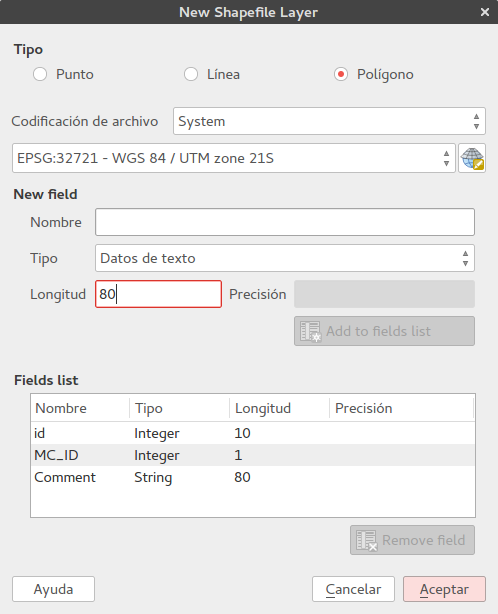
\includegraphics[scale=0.2]{new_shape.png}
\end{center}
\caption{Creacion de una nueva capa vectorial. Se agregan campos que seran de
    interes para comparar las firmas espectrales. }
\label{fig:newshape}
\end{figure}


Una vez creada la nueva capa podemos utilizar la barra de herramientas de qgis
para agregar nuevas geometrias a la misma. Para esto hacemos click en el boton
de agregar geometrica y digitalizamos una zona uniforme dentro de la imagen. 
\begin{figure}
\begin{center}
    
\includegraphics[scale=0.2]{shapetool.png}
\end{center}
\caption{Herramientas de edición vectorial. De izquierda a derecha: 1. Conmutar
    edicion, 2. Guardar cambios a la capa, 3. Añadir objeto espacial, 4. Añadir
    cadena circular, 5. Mover objeto espacial, 6. Herramienta de nodos, 7.
    Borrar lo seleccionado, 8. Cortar objetos espaciales, 9. Copiar objetos
    espaciales, 10. Pegar objetos espaciales.}
\label{fig:shapetool}
\end{figure}

Al terminar de acerlo qgis pedira un numero de ID para la capa que debe ser
correlativo. Además podremos ingresar en este momento los valores del resto de
los campos de nuestro objeto espacial.

\begin{figure}
\begin{center}
    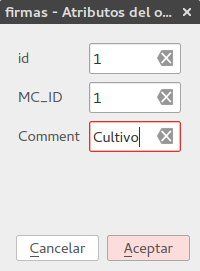
\includegraphics[scale=0.2]{new_poli.png}
\end{center}
    \caption{Valores de los campos del nuevo poligono creado.}
    \label{fig:newpoli}
\end{figure}

\begin{act}
   Digitalize coberturas uniformes dentro de la imagen. Recuerde obtener al
   menos una por cada categoria de uso y cobertura presente dentro de la misma.
\end{act}

En caso de desear cambiar la visualizacion de la capa vectorial, podemos entrar
a las propiedades de la misma\footnote{Pueded utilizar el estilo precargado
ubicado en la carpeta \file{aux\_data}}. Ademas podemos acceder a la tabla de
datos de la capa vectorial haciendo click derecho sobre la misma y eligiendo la
opcion \menu{Abrir tabla de atributos}.

\subsection{Exploracion raster en R}
Busquemos ahora como abrir y trabajar con las imagenes satelitales en R. Para
esto comenzamos cargando las librerias que vamos a utilizar con el comando
\texttt{library(raster)}. 

Además, deberemos situar nuestra carpeta de trabajo donde se encuentran las
carpetas que descargamos. Para esto nos movemos en el explorar de archivos
hasta la misma y hacemos click en usar la carpeta como carpeta de trabajo.

\begin{figure}
\begin{center}
    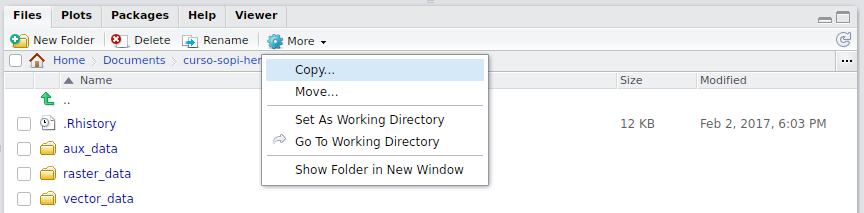
\includegraphics[scale=0.2]{setwd.png}
\end{center}
\caption{Configuracion del directorio de trabajo desde la interfaz grafica.}
\label{fig:setwd}
\end{figure}

Tambien podemos utilizar el comando \texttt{setwd()} para configurar el
directorio de trabajo.

Una vez en dicha carpeta, existen varias maneras de abrir una imagen segun
queramos hacerlo solo para una banda, varias bandas en archivos separados o un
solo archivo multibanda.

Los comandos para esto son \texttt{raster}, para abrir una unica banda,
\texttt{brick}, para abrir un archivo multibanda, y \texttt{stack} para abrir
distinas bandas por separado. Veamos algunos ejemplo de esto:

\begin{exa}
    Abrimos la imagen completa del archivo de Landsat 8 y consultamos sus 
    propiedades. 
    \begin{lstlisting}
    ref.2016 <- brick("raster_data/LC82240782016304/LC82240782016304LGN00.vrt")
    ref.2016
    \end{lstlisting}
    obtenemos de resultado el siguiente text
    \begin{Verbatim}[fontsize=\small]
    class       : RasterBrick 
    dimensions  : 2412, 1834, 4423608, 6  (nrow, ncol, ncell, nlayers)
    resolution  : 30.00402, 30.00265  (x, y)
    extent      : 731118.6, 786146, 7101531, 7173897  (xmin, xmax, ymin, ymax)
    coord. ref. : +proj=utm +zone=21 +south +datum=WGS84 +units=m +no_defs 
                  +ellps=WGS84 +towgs84=0,0,0 
    data source : ./material/raster_data/LC82240782016304/LC82240782016304LGN00.vrt 
    names       : LC82240782016304LGN00.1, LC82240782016304LGN00.2, ... 
    min values  :                     -33,                     192, ... 
    max values  :                    2774,                    3265, ... 
    \end{Verbatim}
    En el podemos ver la clase a la que corresponde el archivo abierto, en este
    caso un \emph{RasterBrick}, las dimensiones, el tamaño de pixel, extension
    de la capa, proyeccion, cual es la ruta al archivo que abrimos, las bandas y
    sus valores maximos y minimos.
\end{exa}

Una vez abierta la imagen en el R podemos empezar a trabajar con la misma
utilizando distintos comandos. 

\begin{exa}
    Veamos primero como cambiar los nombres de las bandas por defecto, cambiar la
    imagen a numeros en reflectancia entre 0 y 1 y luego guardarla nuevamente. Para
    eso ejecutamos el siguiente codigo.
    \begin{lstlisting}
    ref.2016 <- brick(filename)
    names(ref.2016) <- c("blue","gree","red","nir","swir1","swir2")
    ref.2016 <- ref.2016/1e4
    rasterOptions(addheader = "ENVI")
    writeRaster(ref.2016,"raster\_data/processed/ref2016")
    \end{lstlisting}

    Analicemos el codigo linea por linea. 
    \begin{itemize}
    \item La primera de ellas abre la imagen como  un raster de multiples bandas. 
    \item La segunda, cambia los nombres de cada banda a los que figuran en la 
          lista entre parentesis. Es importante resaltar que el numero de nombres 
          debe ser el mismo que el de bandas. 
    \item En tercer lugar convertimos el archivo de numeros enteros entre 0 y 
          10000 a numeros entre 0 y 1.
    \item La cuenta linea es necesaria correrla una sola vez por sesion. La misma
          agrega el header de ENVI a nuestro output para poder abrir el archivo
          desde qgis
      \item La sexta linea guarda el archivo raster con el nombre \file{ref2016} 
    \end{itemize}
    podemos ademas graficar tanto una combinacion de bandas en qgis
    \begin{lstlisting}
    plotRGB(ref.2016,r=4,g=5,b=3, stretch='lin')   
    \end{lstlisting}
    Obtenemos como resultado
    \begin{figure}
    \begin{center}
        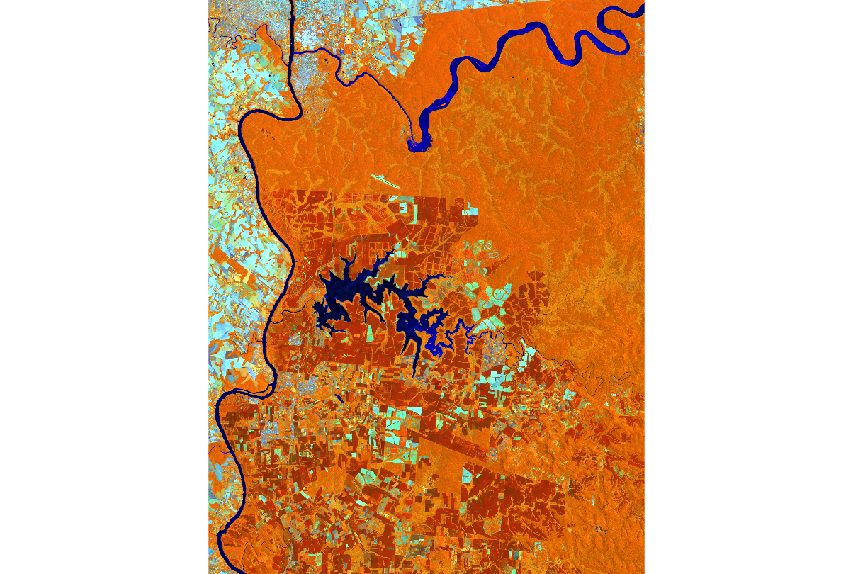
\includegraphics[scale=0.2]{plot453.png}
    \end{center}
    \caption{Combinacion de bandas nir-swir1-red en R.}
    \label{fig:}
    \end{figure}
    como tambien todas las bandas por separado
    \begin{lstlisting}
    plotRGB(ref.2016) 
    \end{lstlisting}
    obtenemos como resultado
    \begin{figure}
    \begin{center}
        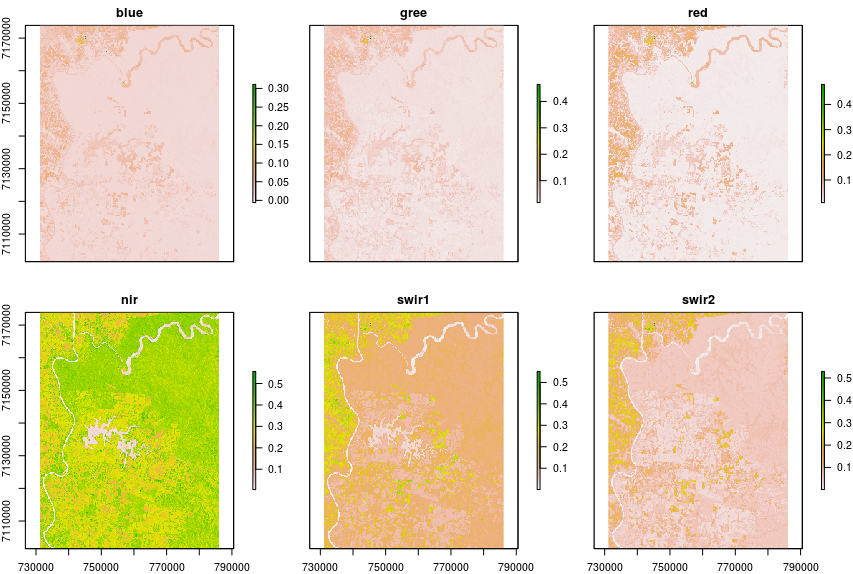
\includegraphics[scale=0.2]{plotband.png}
    \end{center}
    \caption{Grafico de bandas con realce automatico para cada una.}
    \label{fig:plotband}
    \end{figure}
    
\end{exa}
 
\begin{act} 
   Abra el archivo vrt en qgis y vuelva a mirar la firma espectral para 
   distintas coberturas. Entre que valores se encuentra ahora las mismas.
\end{act}

\begin{exa}

    Hagamos un poco de analisis ahora sobre la imagen. En primer lugar podemos
    calcular un sumario de la estadistica de nuestra imagen
    \begin{lstlisting}
    summary(ref.2016)   
    \end{lstlisting}
    obtenemos como resultado
    \begin{Verbatim}[fontsize=\small]
               blue   gree    red     nir   swir1   swir2
    Min.    -0.0278 0.0000 0.0000 -0.0128 -0.0069 -0.0038
    1st Qu.  0.0128 0.0328 0.0184  0.2763  0.1198  0.0493
    Median   0.0138 0.0362 0.0203  0.3287  0.1365  0.0572
    3rd Qu.  0.0170 0.0450 0.0329  0.3557  0.1644  0.0749
    Max.     0.5548 0.8257 0.8034  0.7542  0.9181  0.9446
    NA's     0.0000 0.0000 0.0000  0.0000  0.0000  0.0000
    \end{Verbatim}
    Para comenzar podemos calcular los histogramas de todas las bandas con el 
    comando
    \begin{lstlisting}
    hist(ref.2016) 
    \end{lstlisting}

    y el scatter plot entre dos bandas como

    \begin{lstlisting}
    plot(l8$red, l8$blue)    
    \end{lstlisting}

    en caso de querer todos los scatterplots e histogramas en un solo grafico
    podemos hacerlo con el comando
    \begin{lstlisting}
    pairs(l8)
    \end{lstlisting}
    \end{exa}


\subsection{Manejo vectorial en R}

Hasta ahora estamos analizando la imagen completa. Podemos sin embargo analizar
solo sectores concretos de la imagen muestreandola en funcion de un archivo
vectorial. Tambien sera posible muestrar la imagen pos zonas definidas por otro
raster pero veremos esto mas adelante.

Para poder trabajar con vectores en R utilizaremos la libreria
\texttt{library(rgal)}.

\begin{exa}
    Podemos leer un vector como
    \begin{lstlisting}
    firmas <- readOGR(dsn="vector\_data/", layer="firmas")
    \end{lstlisting}
    Notamos en este caso que debemos indicar por separado la carpeta que
    contiene al shapefilee en \emph{dsn} y el nombre de la capa que queremos
    abrir como \emph{layer}.

    Podemos mostrar las propiedades del vector ejecutando el comando

    \begin{lstlisting}
    vector
    \end{lstlisting}

    obteniendo como resultado
    \begin{Verbatim}[fontsize=\small]
    class       : SpatialPolygonsDataFrame 
    features    : 8 
    extent      : 738692.8, 767774.6, 7133396, 7165265  (xmin, xmax, ymin, ymax)
    coord. ref. : +proj=utm +zone=21 +south +datum=WGS84 +units=m +no_defs
                  +ellps=WGS84 +towgs84=0,0,0 
    variables   : 3
    names       : id, MC_ID,       Comment 
    min values  :  0,     1,          Alto 
    max values  :  9,     8, Suelo desnudo 
    \end{Verbatim}  

    Podemos graficar los vectores obtenidos en R junto aa la imagen de base como

    \begin{lstlisting}
    plotRGB(ref.2016, stretch="lin")
    plot(firmas,add=TRUE,col='red')
    \end{lstlisting}
    donde la primera linea grafica la imagen de fondo y la segunda agrega el
    el shapefile sobre la misma.
\end{exa}

\begin{act} 
    Muestre las propiedades de la capa raster y el vector abiertos y verifique
    que los mismos se encuentren en el mismo sistema de coordenadas.
\end{act}

Por ultimo mostremos como extraer datos de un archivo raster y veamos un par de
ejemplo concretos. La funcion que nos permite extrar datos de un raster segun
un vector es \texttt{extract} que toma dos argumentos
 \begin{lstlisting}
     raster(l8,vector)
 \end{lstlisting}

Veamos algunos ejemplos que pueden ser utiles de aplicacion de todo lo anterior

\begin{exa}
    Graficar en un scatterplot de dos bandas mostrando la zona del espacio 
    ocupada por una cobertura.
 \begin{lstlisting}
    plot(l8$red, l8$nir)
    points(as.data.frame(datos[1])$red, as.data.frame(datos[1])$nir,
    col="green")
 \end{lstlisting}
\end{exa}

\begin{exa}
     Extraer los promedios y desvios standar de un raster y agregarlos a un
     vector.
     \begin{lstlisting}
         promedio <- extract(l8,vector,fun=mean)
         desvio <- extract(l8,vector,fun=sd)
         colnames(promedio) <- paster("mean",colnames("promedio"),sep="_")
         colnames(desvio) <- paster("sd",colnames("desvio"),sep="_")
         vector@data <- cbind(vector@data,promedio,desvio)
         writeOGR(vector, sdn="vector_data/processed/,"datos",driver="ESRI
         Shapefile")
     \end{lstlisting}
\end{exa}

\begin{exa}
     Graficar las firmas espectrales en funcion de la longitud de onda para cada
     geometria de un vector.
     \begin{lstlisting}
         df <- t(promedio)
         colnames(df) <- vector@data$descripcion
         df$wl <- as.matrix(c(485,560,660,830,1650,2215))
         df <- melt(df,id.vars="wl", variable.name="cobertura")
         names(df) <- c("wl","Cobertura","Reflectancia")
         dfd <- t(desvio)
         colnames(dfd) <- vector@data$descripcion
         dfd$wl <- as.matrix(c(485,560,660,830,1650,2215))
         dfd <- melt("wl","Cobertura","Desvio")

         df$desvio <- dfd$desvio

         ggplot(df,aes(wl,Reflectancia)+
            geom_line(aes(colour=Cobertura))+
            geom_poinr(aes(colour=Cobertura))+
            geom_errorbar(aes(ymin=Reflectancia-2*desvio,
                              ymax=Reflectancia+2*desvio))
     \end{lstlisting}
\end{exa}

\begin{act}
    Grafique la media y el desvio standar para las distintas coberturas que pudo
     identificar en el punto uno. 
\end{act}


\chapter{Rebotando por la atm\'osfera}
\label{rebotando}

En esta segunda actividad pr\'actica nos centraremos en la correcci\'on radiom\'etrica
de imagenes satelitales. Son nuestros objetivos:

\begin{itemize}
    \item Abrir una imagen satelital desde el metadato.
    \item Convertir los valores de la imagen a reflectancia tope de la
        atm\'osfera.
    \item Corregir la imagen satelital utilizando los m\'etodos de \emph{dos} y
        \emph{cost}
    \item Corregir la imagen satelital utilizando el \emph{6S} en su versi\'on web.
\end{itemize}

\subsection{C\'alculo de reflectancia a tope de la atmosfera}

Para poder convertir una imagen a reflectancia a tope de la atm\'osfera vamos a
necesitar no solo la imagen sino tambi\'en la informaci\'on adicional que hallaremos
en su metadato.

Para abrir una imagen satelital desde el metadato utilizaremos las funciones
disponibles en la libreria \texttt{RStoolbox}. Esta incluye diversas herramientas
para trabajar con im\'agenes satelitales.

\begin{exa}
    Abramos  la imagen Landsat 7
    del año 2000 desde el metadato y la mostraremos en combinacion color real.
    Adem\'as analicemos sus propiedades.
    \begin{lstlisting}
    meta.2000 <- readMeta("raster_data/LE72240782000188EDC00/LE72240782000188EDC00_MTL.txt")
    \end{lstlisting}
    Podemos mostrar las distintas variables incluidas en el objeto usando el
    signo \$ y su nombre. Por ejemplo \verb|meta.2000$SOLAR_PARAMETERS|
    da como resultado
    \begin{Verbatim}[fontsize=\small]
     azimuth elevation  distance
    37.38251  31.14409   1.01670
    \end{Verbatim}
    Usando el metadato podemos cargar la imagen completa con el comando
    \texttt{stackMeta}. Ademas eliminaremos en este caso las bandas 6 y 7 por
    ser termicas.
    \begin{lstlisting}
    dn.2000 <- stackMeta(meta.2000)
    dn.2000 <- dn.2000[[-6:-7,]]
    dn.2000
    \end{lstlisting}
    obtenemos como resultado un objeto \emph{raster stack} como el que sigue
    \begin{Verbatim}[fontsize=\small]
    class       : RasterStack
    dimensions  : 2412, 1834, 4423608, 6  (nrow, ncol, ncell, nlayers)
    resolution  : 30.00402, 30.00265  (x, y)
    extent      : 731118.6, 786146, 7101531, 7173897  (xmin, xmax, ymin, ymax)
    coord. ref. : +proj=utm +zone=21 +south +datum=WGS84 +units=m +no_defs
                  +ellps=WGS84 +towgs84=0,0,0
    names       : B1_dn, B2_dn, B3_dn, B4_dn, B5_dn, B7_dn
    min values  :     0,     0,     0,     0,     0,     0
    max values  :   255,   255,   255,   255,   255,   255
    \end{Verbatim}
    Mostramos la imagen en cobinaci\'on de color real con \texttt{plotRGB(dn.2000, r=3, g=2, b=1, stretch="lin")}
    obteniendo la figura \ref{fig:dn-l7-rgb}.
     \begin{figure}[h!]
     \begin{center}
         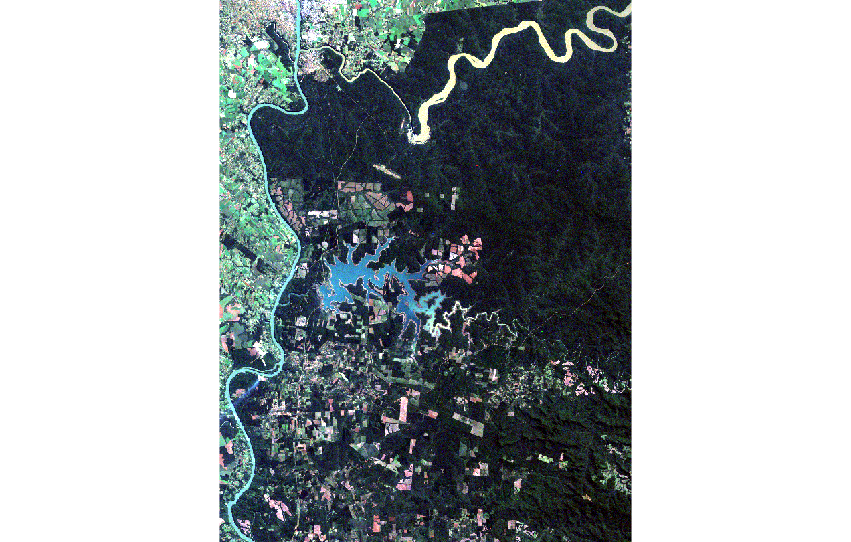
\includegraphics[scale=0.6]{dn-l7-rgb}
     \end{center}
     \caption{Imagen en combinaci\'on de bandas color real de la zona de interes.}
     \label{fig:dn-l7-rgb}
     \end{figure}
\end{exa}

De esta forma tenemos el archivo cargado en n\'umero digital con todos sus metadatos
para convertirlo a reflectancia y realizar distintas correcciones.

Para pasar nuestra imagen a reflectancia a tope
de la atmosfera tenemos dos maneras de hacerlo. Podemos hacerlo a mano
utilizando las herramientas algebraicas de R o podemos hacerlo con la funcion
especifica de \texttt{RStoolbox}.

\begin{exa}
    Calculo de reflectancia a tope de la atm\'osfera
    utilizando el metadato paso por paso

    \begin{lstlisting}
    dn2ref.2000 <- meta.2000$CALREF[1:6,]
    elev.2000 <- pi*meta.2000$SOLAR_PARAMETERS['elevation']/180
    \end{lstlisting}
    extraemos primero del metadatos los par\'ametros de calibraci\'on en
    reflectancia y el \'angulo de elevaci\'on solar. Convertimos luego la imagen
    a reflectancia y la dividimos por el seno del \'angulo solar.
    Luego cambiamos los nombres de las bandas

    \begin{lstlisting}
    toam.2000 <- (dn.2000*dn2ref.2000$gain+dn2ref.2000$offset)/sin(elev.2000)
    names(toam.2000) <- c("blue","green","red","nir","swir1","swir2")
    \end{lstlisting}

    Otra forma de realizar este proceso es utilizando la funci\'on
    \texttt{radCor}. En este caso debemos dar la imagen en DN, el metadato y
    cual es la cantidad que queremos calcular.

    \begin{lstlisting}
    toa.2000 <- radCor(dn.2000, metaData = meta.2000, method = "apref")
    \end{lstlisting}

    Podemos comparar los resultados de ambos metodos inspeccionando los objetos
    \texttt{toam.2000} y \texttt{toa.2000}.
    \begin{Verbatim}[fontsize=\small]
    class       : RasterBrick
    dimensions  : 2412, 1834, 4423608, 6  (nrow, ncol, ncell, nlayers)
    resolution  : 30.00402, 30.00265  (x, y)
    extent      : 731118.6, 786146, 7101531, 7173897  (xmin, xmax, ymin, ymax)
    coord. ref. : +proj=utm +zone=21 +south +datum=WGS84 +units=m +no_defs
                  +ellps=WGS84 +towgs84=0,0,0
    data source : in memory
    names       :        blue,       green,         red,         nir,    swir1,       ...
    min values  : -0.01976113, -0.02181530, -0.02029439,  0.01934678,    -0.02781926, ...
    max values  :   0.6106812,   0.5609009,   0.6079443,   0.8696885,    0.8640919,   ...
    \end{Verbatim}

    y

    \begin{Verbatim}[fontsize=\small]
    class       : RasterStack
    dimensions  : 2412, 1834, 4423608, 6  (nrow, ncol, ncell, nlayers)
    resolution  : 30.00402, 30.00265  (x, y)
    extent      : 731118.6, 786146, 7101531, 7173897  (xmin, xmax, ymin, ymax)
    coord. ref. : +proj=utm +zone=21 +south +datum=WGS84 +units=m +no_defs
                  +ellps=WGS84 +towgs84=0,0,0
    names       :     B1_tre,     B2_tre,     B3_tre,     B4_tre,     B5_tre, ...
    min values  : 0.00000000, 0.00000000, 0.00000000, 0.01934678, 0.00000000, ...
    max values  :  0.6106812,  0.5609009,  0.6079443,  0.8696885,  0.8640919, ...
    \end{Verbatim}

    \end{exa}

\begin{act}
    Inspeccione la reflectancia a tope de la atmosfera para todas las bandas.
    Para esto realice los histogramas, graficos de dispersi\'on, calcule la media,
    el desvio standar y cualquier otra medida estad\'istica que le guste.
\end{act}
\subsection{C\'alculo de reflectancia corregida atmosfericamente por m\'etodos
            estad\'isticos}

La funci\'on \texttt{radCor} dispone de un par\'ametro para hacer distintos
tipos de correcciones atmosf\'ericas. Ya vimos \emph{apref} que nos permiti\'o
calcular la reflectancia a tope de la atm\'osfera. Veamos como aplicar el m\'etodo
de substracci\'on de cuerpo obscuro.

\begin{exa}
    Apliquemos el metodo de \emph{simple dos} para corregir la imagen. En este caso
    solamente restaremos el m\'inimo en cada banda a la imagen para las bandas
    donde existe haze, es decir en la zona del visible y del infrarrojo cercano.

    Estimamos el haze primero y corregimos la imagen luego haciendo
    \begin{lstlisting}
    haze.2000 <- estimateHaze(dn.2000,darkProp = 0.01, hazeBands = 1:4, plot=TRUE)
    sdos.2000 <- radCor(dn.2000, metaData = meta.2000,
                 hazeValues = haze.2000,
                 hazeBands = c("B1_dn","B2_dn","B3_dn","B4_dn"),
                 method="sdos")
    \end{lstlisting}
    en este caso los valores de haze estimados son
    \begin{Verbatim}[fontsize=\small]
    B1_dn B2_dn B3_dn B4_dn
       41    27    20    15
    \end{Verbatim}
    Para hacer un an\'alisis de lo que pasa en la situacion, vamos a graficar los
    histogramas de cada banda para la imagen en reflectancia TOA y corregida por
    el m\'etodo \emph{simple dos}. Para esto usaremos el paquete \texttt{rasterVis}
    \begin{lstlisting}
    B1 <- densityplot(~B1_tre+B1_sre, data=toa.boa, xlab="Reflectancia",
                      ylab="", main="Banda azul", plot.points=FALSE, xlim=c(0,0.3),
                      key=simpleKey(text=c("Tope de la atmosfera",
                                           "Correccion Simple DOS"),
                                           lines=TRUE, points=FALSE))
    B2 <- densityplot(~B2_tre+B2_sre, data=toa.boa, xlab="Reflectancia",
                      ylab="", main="Banda verde", plot.points=FALSE, xlim=c(0,0.3),
                      key=simpleKey(text=c("Tope de la atmosfera",
                                           "Correccion Simple DOS"),
                                           lines=TRUE, points=FALSE))
    B3 <- densityplot(~B3_tre+B3_sre, data=toa.boa, xlab="Reflectancia",
                      ylab="", main="Banda roja", plot.points=FALSE, xlim=c(0,0.3),
                      key=simpleKey(text=c("Tope de la atmosfera",
                                           "Correccion Simple DOS"),
                                           lines=TRUE, points=FALSE))
    B4 <- densityplot(~B4_tre+B4_sre, data=toa.boa, xlab="Reflectancia",
                      ylab="", main="Banda nir", plot.points=FALSE, xlim=c(0,0.3),
                      key=simpleKey(text=c("Tope de la atmosfera",
                                           "Correccion Simple DOS"),
                                           lines=TRUE, points=FALSE))
     print(B1,split = c(1, 1, 2, 2),more=TRUE)
     print(B2,split = c(2, 1, 2, 2),more=TRUE)
     print(B3,split = c(1, 2, 2, 2),more=TRUE)
     print(B4,split = c(2, 2, 2, 2),more=FALSE)
    \end{lstlisting}
    En este caso las primeras 4 funciones crean los histogramas para cada banda
    corregida mientras que las \'ultimas 4 lineas los imprimen en una grilla como
    se ve en la figura \ref{fig:simpledos}.
    \begin{figure}[h!]
    \begin{center}
        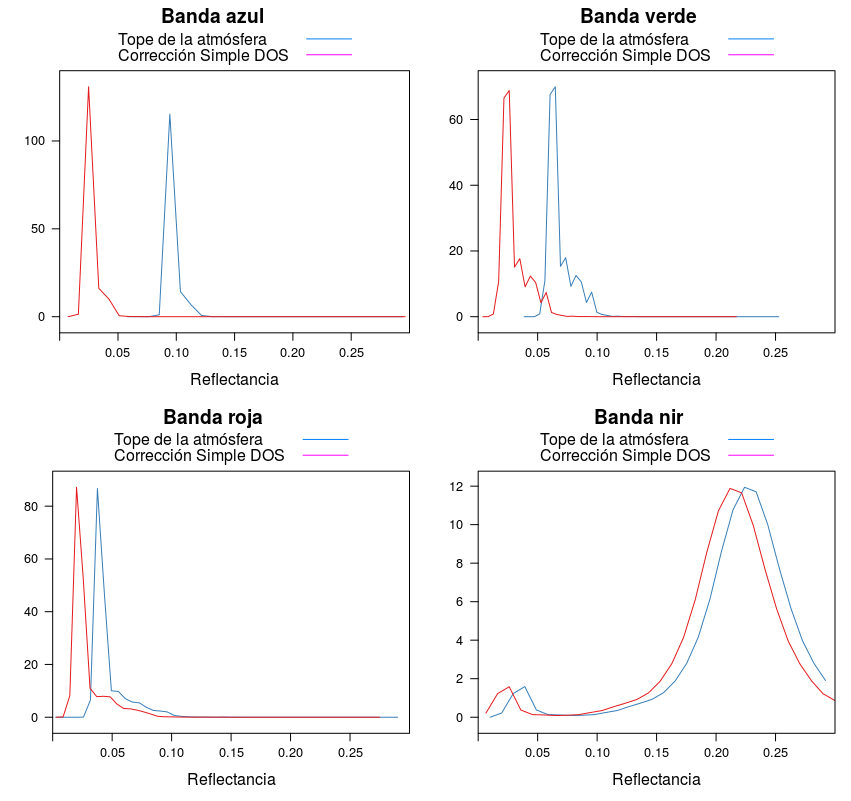
\includegraphics[scale=0.4]{simpledos.png}
    \end{center}
    \caption{Graficos de densidad para las distintas bandas donde se
        muestra el nivel de correcci\'on en cada una.}
    \label{fig:simpledos}
    \end{figure}
Notamos en este caso que la correccion se vuelve menos importante a medida
que crece la longitud de onda. adem\'as, la corecci\'on solo cambia la
posici\'on de la distribuci\'on y no su forma.

\end{exa}
\begin{act}
    Analice los valores de haze obtenidos por la funcion stimate haze y grafiquelos
    como funci\'on de la longitud de onda en escala logaritmica. ¿Que observa?
\end{act}

\begin{act}
    Utilice el m\'etodo \emph{costz} para corregir la imagen a reflectancia a tope
    de la superficie. Puede ayudarse con el comando \texttt{?radCor}
\end{act}

\begin{act}
    Guarde el archivos raster generado por cada uno de los m\'etodos de
    correcci\'on. Abralos en QGIS y comparelos visualmente. Obtenga firmas
    espectrales con los distintos m\'etodos de correccion.
\end{act}


\subsection{6S}
\label{sub:corr:6S}

Veamos ahora como operar con el 6S para obtener una estimaci\'on de los par\'ametros
atmosf\'ericos. Para esto utilizaremos la versi\'on web del 6S que se encuentra
disponible en \url{http://6s.ltdri.org/pages/run6SV.html}.

Para utilizarla ingresaremos a la pagina y haremos click en el boton
\menu{Submit query}. Iremos luego configurando paso a paso nuestro modelo de la
atm\'osfera haciendo siempre luego click en el bot\'on \menu{submit query} para
pasar al paso siguiente.

Los parametros para nuestro modelo son

\begin{enumerate}
    \item Geometrical conditions
        \begin{itemize}
            \item TM (Landsat)
            \item Month: 4, Day:13, GTM decimal hour: 13.60, Longitude:
                -63.8606, Latitude: -24.9937.
        \end{itemize}
    \item Atmospheric Model
        \begin{itemize}
            \item Select Atmospheric Profile: Mid latitude summer
            \item Select aerosol model: Continental Model
            \item Visibility: 60
        \end{itemize}
    \item Target \& sensor altitude
        \begin{itemize}
            \item Select targe altitude: sea level
            \item Select sensor altitude: satellite level
        \end{itemize}
    \item Spectral conditions
        \begin{itemize}
            \item Select spectral conditions: choose band
            \item Select band: 1st band of tm (landat 5)
        \end{itemize}
    \item Ground reflectance
        \begin{itemize}
            \item Ground reflectance type: homogeneous surface
            \item Directional effect: no directional effect
            \item Specify surface reflectance: input constant value of ro
            \item input constant value for ro: 0
        \end{itemize}
    \item Signal
        \begin{itemize}
            \item Atmospheric correction mode: no atmospheric correction
        \end{itemize}
\end{enumerate}

Todos estos valores los encontramos en el metadato de la imagen.

En \menu{7.Results} podemos ver el resultado haciendo click en \emph{Output
file}. Del mismo debemos extraer los valores de
 \begin{itemize}
     \item \texttt{global gas. trans. - total}
     \item \texttt{total sca. trans. - total}
     \item \texttt{spherical albedo - total}
     \item \texttt{reflectance I - total}
 \end{itemize}

Una vez ejecutado el proceso puede usarse el siguiente c\'odigo para corregir
todas las bandas utilizando R.

\begin{lstlisting}
    a <- c(0.98,0.90,...) # Global gas transmitance
    b <- c(0.81,0.90,...) # Total scatering transmitance
    g <- c(0.15,0.10,...) # Spherical albedo
    r <- c(0.08,0.05,...) # Reflectance I
    sss.2000 <- (toa.2000/(a*b)-r/b)/(1+g*(toa.2000/(a*b)-r/b))
\end{lstlisting}


\begin{act}
    Realice una extracci\'on de firmas espectrales para distintass coberturass de
    cada uno de los archivos raster obtenidos y grafiquelos juntas.
    Comparela con la firma espectral obtenida a partir de la imagen corregida
    por el usgs.
\end{act}

\begin{act}
    Haga un gr\'afico de densidades que muestre los distintos m\'etodos de
    correcci\'on atmosf\'ericos para cada banda.
\end{act}

\begin{act}
    Calcule la diferencia promedio para cada banda entre las imagenes en
    reflectancia a tope de la atmosfera y las distintas correcciones
    y la imagen en reflectancia entregada por el USGS.
\end{act}


\chapter{Un \'abaco espectral}
\label{abaco}
Veamos ahora como realizar operaciones sencillas entre las bandas de una imagen.
Usaremos en esta practica los siguientes paquetes

\begin{lstlisting}
    library(raster)
    library(RStoolbox)
    library(RColorBrewer)
    library(rgdal)
    library(ggplot2)
    libyrary(GGally)
\end{lstlisting}

Comenzamos primer cargando la imagen desde el metadato y convirtiendola a
reflectancia como hicimos en la clase anterior

\begin{lstlisting}
    xml.2016 <- readMeta("raster_data/LC.../LC....xml")
    ref.2016 <- stackMeta(xml.2016, quantity = "sre")
    scaleF <- getMeta(ref.2015,xml.2016, what = "SCALE_FACTOR")
    ref.2016 <- ref.2016 * scaleF
    ref.2016 <- ref.2016[[-1,]]
    names(ref.2016) <- c("blue","green","red","nir","swir1","swir2")
\end{lstlisting}

una vez cargada la imagen podemos realizar operaciones entre las bandas llamando
a cada una por separado. Veamos como ejemplo el calculo de NDVI\@.

\begin{exa}
    Calculo de NDVI a mano y grafico del mismo
    \begin{lstlisting}
        ndvi.2016 <- (ref.2016$nir-ref.2016$red)/(nir.2016$nir+ref.2016$ref)
        cols = colorRampPalette(brewer.pal(9,"YlGn"))(16)
        plot(ndvi.2016, col=cols, zlim = c(0,1))
    \end{lstlisting}
    obteniendo una imagen como la que se ve debajo.
\end{exa}

El paquete \texttt{RStoolbox} tiene varias herramientas que nos ayudan a
calcular los indices espectrales. Veamos por ejemplo como calcular el NDVI y el
EVI utilizando dicho paquete

\begin{exa}
    Para calcular los indices mediante la funcion spectralIndices debemos
    especificar con que raster trabajamos y que bandas corresponden a cada
    longitud de onda
    \begin{lstlisting}
    indices.2016 <- spectralIndices(ref.2016, 
                                    blues="blue", red="red", nir="nir", 
                                    indices=c("NDVI","EVI"))
    plot(indices.2016,col=cols, zlim=c(0,1))
    \end{lstlisting}
    obtenemos una imagen como se muestra debajo.
\end{exa}

\begin{act}
    Calcule el NDVI para el año 2000 utilizando la imagen landsat 7.
\end{act}

\begin{act}
    Calcule y grafique todos los indices posibles que involucren a las bandas
    roja y nir de landsat 8. 
\end{act}


\begin{exa}
    Veamos ahora como calcular el tSAVI utilizando la linea de suelo obtenida a
    partir de la imagen. Para esto necesitaremos enmascarar las zonas con
    cobertura de agua y nubes. Veamos primer como hacer esto.
    \begin{lstlisting}
        mask.2016 <- raster("raster/.../...cfmask.tif")
        masked.2016 <- mask(ref.2016, mask=mask.2016, inverse=TRUE,
                            maskvalue=0, updatevalue=255)
        masked.2016[masked.2016<=0] <- 255
    \end{lstlisting}
    de esta forma enmascaramos todos los valores con nubes, agua y donde la
    reflectancia obtenida es cero.
    Calculamos ahora la linea de suelo y la mostramos en un scatterplot
    \begin{lstlisting}
        bsl.2016 <- BSL(as.matrix(masked.2016$red), as.matrix(masked.2016$nir),
                        method="quantile", ulimimt=0.99, llimit=0.001)
        plot(ref.2016$red, ref.2016$nir)
        abline(bsl.2016$BSL,col="red")
    \end{lstlisting}
\end{exa}

\begin{act}
    Calcule el tSAVI utilizando la linea de suelo obtenida arriba.
\end{act}

\begin{act}
    Vuelva a obtener la linea de suelo sin enmascarar la imagen y dibujo el
    scatterplot con la misma y la anterior. Que problema encuentra.
\end{act}

Finalmente, veamos como se puede obtener datos biofisicos a partir de los
indices de vegetacion calculados. De esta forma podremos generar mapas de
porcentaje de cobertura, productividad, etc.

\begin{act}
    Cargue la capa vectorial del muestreo de variables biofisicas
    \texttt{muestreo.shp} y haga una extraccion de los valores de NDVI
    correspondientes a dichos puntos. Guarde estos valores en un dataframe
    llamado \texttt{muestreo}.
\end{act}

\begin{exa}
    Veamos como ajustar con R un modelo lineal a nuestro modelo. Para esto
    comencemos haciendo un analisis visual con la funcion \texttt{ggpairs}.
    \begin{lstlisting}
        ggpairs(muestreo,diag=list(continuous="barDiag"))
    \end{lstlisting}
    Obtendremos un grafico que presenta los scatterplots entre las bandas, su
    correlacion e histogramas.
    Veamos en el mismo que la superficie cubierta por vegetacion varia
    linealmente con el NDVI\@. Por lo tanto utilizaremos estos para hacer un
    ajuste de nuestro modelo.
    \begin{lstlisting}
        lm.2016 <- lm(fcover~ndvi, data=muestreo)
        plot(muestreo$ndvi, mustreo$fcover)
        abline(lm.2016, col="red")
        summary(lm.2016)
    \end{lstlisting}
    de esta forma veremos los parametros de nuestro ajuste, y graficaremos al
    mismo en un scatterplot.

    Para aplicar el modelo a nuestro raster hacemos
    \begin{lstlisting}
        fcover.2016 <- predict(ndvi.2016,lm.2016)
        plot(fcover.2016)
    \end{lstlisting}
    Obteniendo el mapa de abajo.
\end{exa}

\begin{act}
    Genere los modelos de lai, fapar y fcover para el año 2016 y con los mismos
    realice mapas de dichas variables.
\end{act}

\begin{act}
    Utilizando los modelos obtenidos para 2016 aplique los mismos para obtener
    los mapas de lai, fapar y fcover del año 2000. Que suposicion esta
    haciendo?
\end{act}

\begin{act}
    * Utilizando la funcion spectralIndices y ggpairs, analice si hay otro indice
    que ajuste que correlacione mejor con las alguna de las varibles biofisicas
    medidas a campo.
\end{act}



\part{Variables discretas}

\chapter{Geometr\'ia espectral}
\label{rotaciones}
En nuestra cuarta pr\'actica trabajemos con rotaciones en el espacio espectral.
Apuntamos a poder incorporar conceptos como dimensionalidad y
correlaci\'on entre bandas, que nos ayuden a utilizar mejor la informaci\'on
satelital.

Son nuestros objetivos:

\begin{itemize}
    \item Aplicar la transformada tasseled cap a una imagen multiespectral e
        interpretar el significado de cada banda.
    \item Aplicar la transformada por componentes principales a una imagen
        multiespectral e interpretar el resultado.
    \item Aplicar la transformada por componentes principales a un stack
        de bandas multiespectrales de distintas fechas e interpretar los resultados.
    \item Extraer informaci\'on de series temporales de \'indices espectrales.
\end{itemize}

\subsection{C\'alculo de la transformada tasseled cap para una imagen landsat}

Comencemos calculando la transformada tasseled cap para una imagen Landsat 8. \'Esta
ser\'a la primer rotaci\'on que utilizaremos en el curso cuya la
interpretaci\'on es bastante sencilla. Usaremos el paquete
\texttt{RStoolbox}.

\begin{exa}
    Para cualcular la transformada por componentes principales comenzamos
    abriendo la imagen Landsat 8 desde el metadado y convirti\'endola a reflectancia
    a tope de la cobertura, como vimos en las clases anteriores.
    \begin{lstlisting}
    xml.2016 <- readMeta("raster_data/LC82240782016304/LC82240782016304LGN00.xml")
    ref.2016 <- stackMeta(xml.2016, quantity = "sre")
    scaleF <- getMeta(ref.2016,xml.2016, what = "SCALE_FACTOR")
    ref.2016 <- ref.2016 * scaleF
    ref.2016 <- ref.2016[[-1,]]
    names(ref.2016) <- c("blue","green","red","nir","swir1","swir2")
    \end{lstlisting}

    Analizamos ahora el espacio rojo-infrarrojo cercano y rojo-verde para la imagen

    \begin{lstlisting}
    B1 <- xyplot(nir~red,data=ref.2016)
    B2 <- xyplot(red~green,data=ref.2016)
    print(B1,split=c(1,1,2,1),more=TRUE)
    print(B2,split=c(2,1,2,1),more=FALSE)
    \end{lstlisting}

    obteniendo como scatterplots (Figura \ref{fig:green-red}).

    \begin{figure}[h!]
    \begin{center}
        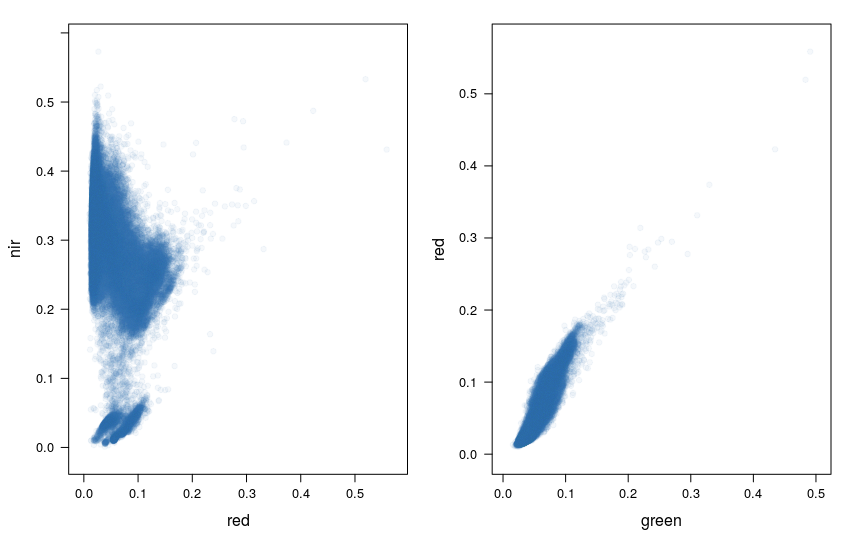
\includegraphics[scale=0.6]{red-nir-green.png}
    \end{center}
    \caption{Scatterplot verde-rojo y nir-red.}
    \label{fig:green-red}
    \end{figure}

    Calculemos ahora la transformada tasseled cap. Para eso usamos la funci\'on
    \texttt{tasseledCap} del paquete \texttt{RStoolbox}.
    \begin{lstlisting}
    tsc.2016 <- tasseledCap(ref.2016,sat="Landsat8OLI")
    \end{lstlisting}
    Tendremos una imagen de tres bandas, \emph{brillo}, \emph{verdor} y
    \emph{humedad}. Podemos graficar cada una de las bandas por separado con el
    comando \texttt{plot(tsc.2016)} o todas juntas con \texttt{plotRGB(tsc.2016,r=1,g=2,b=3, stretch="lin")}
\end{exa}

\begin{act}
    Calcule la transformada tasseled cap para la imagen Landsat 7 del año 2000.
\end{act}

\subsection{C\'alculo de la transformada por componentes principales}

Veamos ahora como calcular la transformada por componentes principales. Utilizaremos la
herramienta \texttt{rasterPCA} del paquete \texttt{RStoolbox}.

\begin{exa}
    Comencemos analizando la transformada por componentes principales de la
    imagen de 2016. Miremos primero los scatterplots con el comando \texttt{pairs(ref.2016)}
    obteniendolos (Figura \ref{fig:pairs2})
    \begin{figure}[h!]
    \begin{center}
        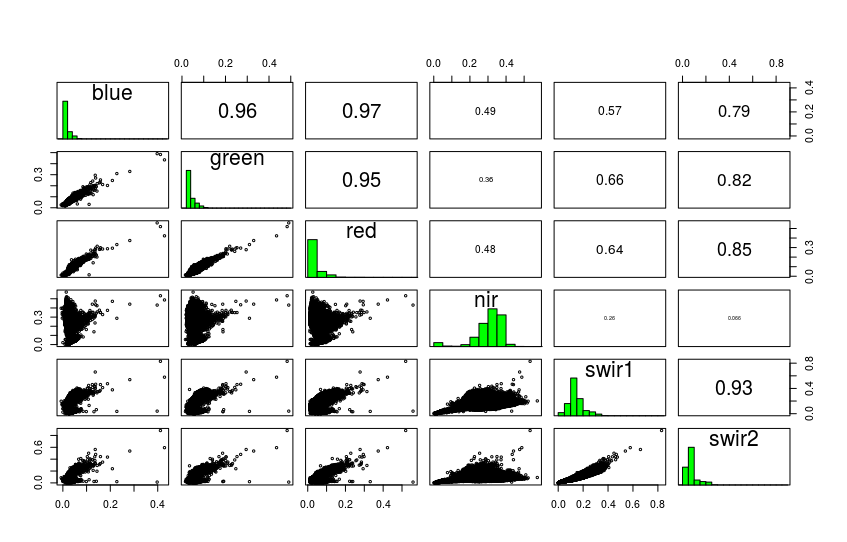
\includegraphics[scale=0.4]{pairs.png}
    \end{center}
    \caption{Scaterplots y coeficientes de correlaci\'on para la imagen Landsat 8.}
    \label{fig:pairs2}
    \end{figure}

    Mirando el resumen de la imagen vemos que hay varias bandas muy
    correlacionadas entre s\'i, como las del visible, mientras que otras lo
    estan poco, como el infrarrojo cercano y el infrarrojo de onda corta. Por lo tanto, esperamos que no
    todas las bandas sean necesarias para explicar el comportamiento de la
    imagen, al menos en el nivel de detalle m\'as bajo.

    Apliquemos entonces la transformada por componentes principales y veamos que
    sucede

    \begin{lstlisting}
        pca.2016 <- rasterPCA(ref.2016)
        summary(pca.2016$model)
    \end{lstlisting}

    El sumario del modelo obtenidos,
    \begin{Verbatim}[fontsize=\small]
    Importance of components:
                               Comp.1     Comp.2     Comp.3      Comp.4 ...
    Standard deviation     0.08079854 0.07808556 0.01242745 0.006488765 ...
    Proportion of Variance 0.50850204 0.47492732 0.01202957 0.003279516 ...
    Cumulative Proportion  0.50850204 0.98342936 0.99545892 0.998738441 ...
    \end{Verbatim}

    Al observar las varianzas, vemos que las 3 primeras explican m\'as que el
    99.5\% de la variabilidad de la imagen. Es decir que, de las 6 bandas de
    Landsat 8 en esta imagen, 3 nos alcanza para explicar casi todo el
    comportamiento. Analisemos la primera, usando el comando
    \texttt{loadings(pca.2016\$model)} para ver como son las componentes.

    \begin{Verbatim}[fontsize=\small]
    oadings:
          Comp.1  ...
    blue
    green
    red   -0.128  ...
    nir   -0.575  ...
    swir1 -0.663  ...
    swir2 -0.451  ...
    \end{Verbatim}

    La primer componente pesa siempre con el mismo signo, a
    todas las bandas. Podemos interpretarla como un
    brillo negativo y esperar que sea m\'as alta cuando miramos zonas de la imagen que
    tengan menos reflectancia en promedio. La segunda componente, presenta diferencia
    entre los valores del infrarrojo cercano y el resto de la bandas. Esta ser\'a alta
    en presencia de vegetaci\'on y baja en su ausencia. La componente tres se comporta
    de forma similar pero con las bandas del infrarrojo medio, por lo tanto podemos
    interpretarla como una componente que varia seg\'un el contenido de humedad.
\end{exa}

\begin{act}
    Calcule y analice la transformada por PCA de la imagen Landsat 7 del año
    2000.
\end{act}

\subsection{Algunas ideas sobre series temporales}

Empecemos esta seccion con una actividad

\begin{act}
    Aplique la transformada por componentes principales al stack de bandas del
    año 2000 y 2016.
\end{act}

Veamos que pasa al trabajar con series temporales de \'indices.

\begin{exa}
    Otra aplicaci\'on de la transformada por componentes principales
    es el an\'alisis de series temporales.
    \begin{lstlisting}
    ndvi.list <- list.files("raster_data/MOD13Q1/NDVI/", pattern = "*.tif$",
                             full.names = TRUE)
    ndvi.stack <- stack(ndvi.list)
    \end{lstlisting}
    una vez abierta la imagen la convertimos a valores entre -1 y 1 e
    interpolamos los valores faltantes.
    \begin{lstlisting}
    ndvi.stack <- ndvi.stack/1e4
    ndvi.stack <- approxNA(ndvi.stack)
    writeRaster(ndvi.stack,"ndvi-series.tif")
    \end{lstlisting}
    Una vez interpoladas las fechas donde no hab\'ia datos de NDVI, podemos
    abrirla en el QGIS y analizar distintas zonas de la imagen.

    Utilizando la herramienta de identificar objetos espaciales podemos
    consultar como es el comportamiento de la serie temporal para cada p\'ixel.

    \begin{figure}[h!]
    \begin{center}
        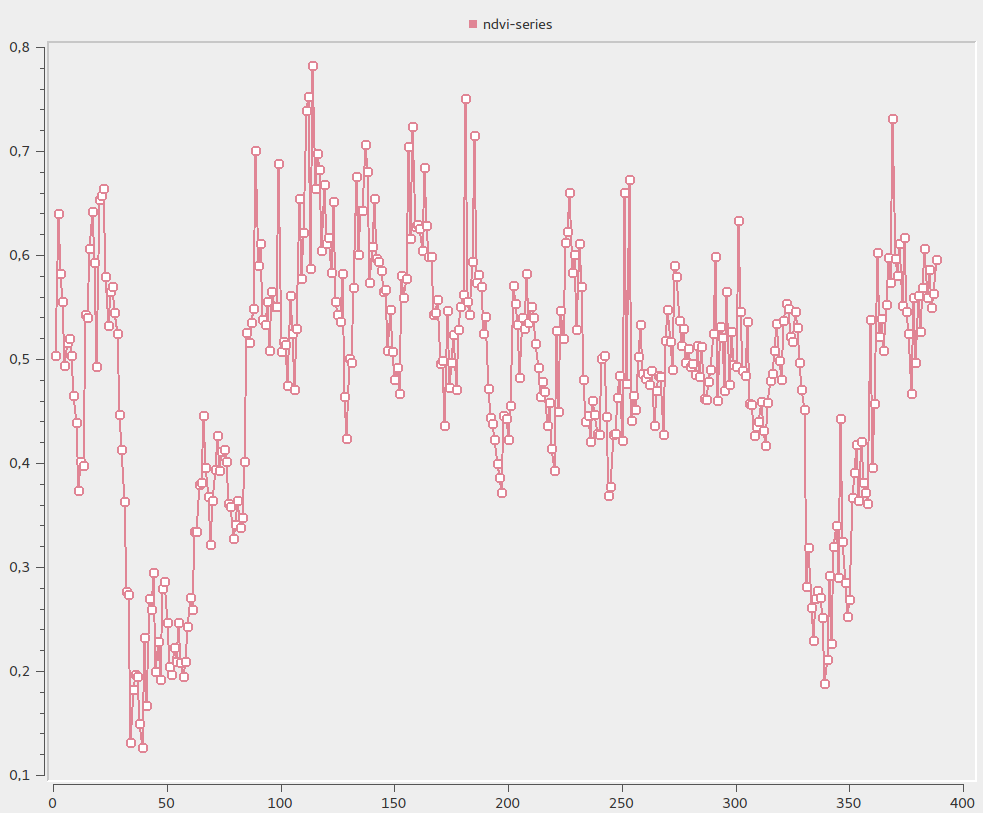
\includegraphics[scale=0.3]{series.png}
    \end{center}
    \caption{Serie temporal de valores de NDVI.}
    \label{fig:series}
    \end{figure}

    Vemos que distintas zonas tienen distintos comportamientos intra e
    interanual.

    Podemos analizar el promedio y el desv\'io standar para cada p\'ixel de la
    imagen
    \begin{lstlisting}
    ndvi.mean <- mean(ndvi.stack)
    plot(ndvi.mean)
    ndvi.sd <- calc(ndvi.stack, fun=sd)
    plot(ndvi.sd)
    \end{lstlisting}
\end{exa}


\begin{act}
    Grafique las primeras 4 componentes de la transformada por componentes
    princiales de la imagen del stack de NDVI\@. ¿Qu\'e zonas puede identificar en la
    primera? ¿Qu\'e zonas se distinguen en la segunda? ¿Qu\'e comportamiento encuentra
    en la tercera y cuarta?
\end{act}


\chapter{Clasificacion no supervisada de imagenes}
\label{otrolado}
En la quinta clase del curso, trabajaremos con clasificaci\'on no supervisada
de im\'agenes satelitales. Son nuestros objetivos:

\begin{itemize}
  \item Usar la herramienta de clasificaci\'on no supervisada.
  \item Aprender a indentificar clases espectrales en catego\'ias de uso y cobertura.
  \item Incorporar informaci\'on no espectral a las clasificaciones como
  pueden ser datos temporales o informaci\'on espacial.
  \item Aplicar la transformada por componentes principales para reducir la dimensionalidad
  y seleccionar los datos mas relevantes previos a las clasificaciones.
\end{itemize}

\subsection{Clasificaci\'on mediante el m\'etodo k-means}

Cargaremos primero la imagen landsat 8 y habilitaremos la opcion para escribir
el header de ENVI\@.

\begin{lstlisting}
    rasterOptions(addheader = "ENVI")
    xml.2016 <- readMeta("raster_data/LC82240782016304/LC82240782016304LGN00.xml")
    ref.2016 <- stackMeta(xml.2016, quantity = "sre")
    scaleF <- getMeta(ref.2016,xml.2016, what = "SCALE_FACTOR")
    ref.2016 <- ref.2016 * scaleF
    ref.2016 <- ref.2016[[-1,]]
    names(ref.2016) <- c("blue","green","red","nir","swir1","swir2")
\end{lstlisting}

Veamos como clasificar una imagen usando el m\'etodo k-means en R. Vamos a usar
los paquetes \texttt{raster} y \texttt{RStoolbox}

\begin{exa}
    Comenzamos seteando la semilla para el geneador de n\'umeros aleatorios con el
    comando \texttt{set.seed(42)}. De esta forma la serie de n\'umeros aleatorios
    es la misma para todos.

    Luego clasificamos la imagen y la guardamos como vimos en las clases anteriores.
    \begin{lstlisting}
    kmeans.2016 <- unsuperClass(ref.2016, nClasses = 5, nStarts = 100,
                                nSamples = 100)
    writeRaster(kmeans.2016, "raster_data/processed/kmeans2016",
                datatype="INT1U")
    \end{lstlisting}

    En este caso estamos solamente usando 5 clases espectrales.

    Podemos ahora graficar por separado cada una de las clases
    \begin{lstlisting}
        clases.2016 <- layerize(kmeans.2016)
        plot(clases.2016)
    \end{lstlisting}

    Abriremos la imagen ahora en el qgis e identificaremos cada una de las clases
    realiando interpretacion visual de la imagen.

    Para realizar la identificacion primero vamos al menu \menu{propiedades de la
    imagen, Estilo, Tipo de renderizacion, Unibanda pseudocolor}. Elegimos de modo
    Intervalo Igual y en numero de clases ponemos con el minimo en 1 y el maximo en
    100. En estilo de color elegimos colores aleatorios. Iremos luego cambiando los
    colores uno a uno por un color brillante e identificado a que cobertura
    pertenece dicha clase espectral.

    Construiremos con ella una tabla como la siguiente

\begin{verbatim}
    id  class
    1   1
    2   1
    3   2
    4   5
    5   7
\end{verbatim}

que guardaremos en un archivo de texto. El mismo lo utilizaremos para realizar
la fusion de clases.

Una vez conocidas las categorias de uso y cobertura correspondientes a cada
clase espectral podemos combinarlas

\begin{lstlisting}
    clases.2016 <- read.delim("class")
    reclas.2016 <- subs(kmeans.2016$map, clases.2016)
\end{lstlisting}

\end{exa}
\begin{act}
    Clasifique por el metodo de kmeans la imagen en reflectancia con una
    cantidad de clases espectrales lo suficientemente altas para separar todas
    las clases espectrales.
\end{act}

\begin{act}
    Vuelva a repetir la clasificacion utilizando la imagen obtenida de la
    transformada por componentes principales descartando las bandas que aporten
    menos informacion.
\end{act}

Podemos ahora utilizar la clasificacion para separar zonas de la imagen en el
espacio espectral

\begin{lstlisting}
    ref.2016$kmeans <- reclas.2016
    xyplot(nir~red, groups=kmeans, data=ref.2016)
\end{lstlisting}

\begin{act}
    Grafique en los cortes del espacio espectral la imagen sin fusionar. Compare
    la diferencia entre clases espectrales y clases de informacion.
\end{act}


\chapter{Clasificacion supervisada de imagenes}
\label{educando}
En la sexta clase del curso, continuamos trabajando con algor\'itmos de clasificaci\'on
de im\'agenes, centrandonoces ne este caso en los no supervisados. Son nuestros objetivos:

\begin{itemize}
  \item Poder realizar clasificaciones no supervisadas utilizando los distintos
  algoritmos que se encuentran en R.
  \item Calcular la distancia espectral entre como forma de determinar la separabilidad
  de dos clases espectrales.
  \item Comparar utilizando la entropia de un pixel que coberturas presentan
  mayor confusion al momento de la clasificacion.
\end{itemize}

Cargaremos primero la imagen landsat 8 y habilitaremos la opcion para escribir
el header de ENVI\@. Usaremos en primer lugar los paquetes \texttt{raster},
\texttt{rgdal} y \texttt{RStoolbox}.

\begin{lstlisting}
    rasterOptions(addheader = "ENVI")
    xml.2016 <- readMeta("raster_data/LC82240782016304/LC82240782016304LGN00.xml")
    ref.2016 <- stackMeta(xml.2016, quantity = "sre")
    scaleF <- getMeta(ref.2016,xml.2016, what = "SCALE_FACTOR")
    ref.2016 <- ref.2016 * scaleF
    ref.2016 <- ref.2016[[-1,]]
    names(ref.2016) <- c("blue","green","red","nir","swir1","swir2")
    vector <- readOGR(dsn="vector_data/", layer="entrenamiento")
\end{lstlisting}

\subsection{Clasificador por m\'axima verosimilitud}

Empecemos con la clasificacion por el metodo de maxima verosimilitud, para esto
necesitamos del paquete

\begin{lstlisting}
    sup.2016 <- superClass(ref.2016, vector, responseCol = "MC_ID",
                           model = "mlc")
    plot(sup.2016, col=rainbow(8))
\end{lstlisting}

y realizar el scatterplot de dichas variables como.

\begin{lstlisting}
    ref.mlc <- stack(ref.2016,sup.2016$map)
    xyplot(nir~red, groups=MC_ID , data=ref.mlc)
\end{lstlisting}

Cambiando el algoritmo de clasificacion en el parametro \texttt{model} podemos
calcular distintas clasificaciones supervisadas. Algunas de las vistas en clase
son \texttt{rf}, \texttt{svmRadial}, \texttt{kNN}. Cada una de ellas usa alguna
libreria adicional de las cargadas antes.

\begin{exa}
  Una forma de mejorar las clasificaciones supervisadas basadas en el espacio
  espectral es clasificar por separado distintas clases espectrales y luego unirlas
  en la misma clase de informacion. Veams como hacerlo.
  \begin{lstlisting}
      sup.2016b <- superClass(ref.2016, vector, responseCol = "C_ID",
                             model = "mlc")
  \end{lstlisting}

  Una vez realizada la clasificacion, debemos substituir los valores de cada pixel
  por el de la clase de informacion correspondiente. Para ello hacemos

  \begin{lstlisting}
    subs.2016 = vector@data[c(3,1)]
    sub.2016 <- reclassify(sup.2016b$map, subs.2016)
    writeRaster(sub.2016, "raster_data/processed/mlc2016",
                datatype="INT1U")
    plot(sub.2016, col=rainbow(8))
  \end{lstlisting}


    Podemos finalmente comparar las dos imagenes clasificadas lado a lado ejecuntado el
    comando \verb|plot(stack(sup.2016$map,sub.2016),col=rainbow(8))|
\end{exa}

\begin{act}
    Realice clasificaciones por los distintos metodos y comparelas visualmente.
\end{act}

\begin{act}
    Agregue las bandas de textura y evolucion temporal del NDVI y vuelva a clasificar
    las imagenes.
\end{act}

\subsection{Entropia de la clasificacion}

Para poder comparar en que zonas los clasificadores presentan mas o menos
dispersion podemos calcular la entropia de las distintas clasificaciones en cada
pixel. Para esto utilizaremos la funcion \texttt{rasterEntropy}.

\begin{exa}
  Para esto comenzamos corriendo la clasificacion para distintos modelos, los apilados y
  despues calculamos la entropia de los mismos

  \begin{lstlisting}
      set.seed(42)
      sup.2016 <- superClass(ref.2016, vector, responseCol = "C_ID",
                           model = "mlc")
      mlc.2016 <- reclassify(sup.2016$map, subs.2016)

      library(randomForest)
      sup.2016 <- superClass(ref.2016, vector, responseCol = "C_ID",
                           model = "rf")
      rf.2016 <- reclassify(sup.2016$map, subs.2016)

      library(kernlab)
      sup.2016 <- superClass(ref.2016, vector, responseCol = "C_ID",
                           model = "svmLinear")
      svm.2016 <- reclassify(sup.2016$map, subs.2016)

      prediction_stack <- stack(mlc.2016, rf.2016, svm.2016)
      names(ensemble) <- c("mlc","rf","svm")

      model_entropy <- rasterEntropy(prediction_stack)
  \end{lstlisting}

  Podemos graficar la entropia de las clasificaciones como \verb|model_entropy|
  y ver que zonas presentan mas diferencias a la hora de la clasificacion y cuales no.
  \begin{lstlisting}
    plot(stack(prediction_stack, model_entropy),col=rainbow(8))
  \end{lstlisting}
\end{exa}

\begin{act}
  Repita las clasificaciones por los metodos de arriba agregando la banda
  textura y de variacion temporal del ndvi. Apilela junto con las clasificaciones por
  k-means de la clase anterior. ¿A que cobertura pertenecen las zonas con mayor
  variabilidad?
\end{act}


\chapter{Tecnicas pos-clasificacion}
\label{pos}
Veamos finalmente, en esta pr\'actica, algunas t\'ecnicas de posprocesamiento
para im\'agenes satelitales que nos ayudaran a mejorar los valores extraidos
y conocer la incerteza en su estimaci\'on. Son nuestros objetivos:

\begin{itemize}
  \item Aplicar filtros modales a las clasificaciones para eliminar p\'ixeles
  aislados.
  \item Poder calcular la presici\'on total para la clasificaci\'on y sus precisiones
  del usuario y productor.
  \item Estimar el error de para las areas calculadas a partir de la imagen
  clasificada.
\end{itemize}

Vamos a usar los paquetes \texttt{raster}, \texttt{rgdal}, \texttt{RStoolbox} y
\texttt{rasterVis}.

\subsection{Filtrado de clasificaciones}

Una de las primeras tareas a realizar luego de clasificar una imagen es
aplicar un filtro a la misma que permite eliminar p\'ixeles aislados. Al
hacerlo podremos descartar, por ejemplo, pixeles de ciudad en el medio de la selva
o de selva en medio de la ciudad. Esta es otra forma de incorporar el contexto
espacial a nuestras clasificaciones
\begin{exa}
  Veamos como aplicar un filtro por moda a una imagen clasificada.

  Comencemos cargando una imagen clasificada en R
  \begin{lstlisting}
      mlc.2016 = raster(raster_data/processed/mlc2016)
  \end{lstlisting}

  Para aplicar el filtro de 3x3 creamos una matriz con unos de 3x3 y usamos
  el comando \texttt{focal} con la funcion \texttt{modal}

  \begin{lstlisting}
      window <- matrix(1,nrow=3, ncol=3)
      mlc.3x3<-focal(mlc.2016,w=window,fun=modal)
      writeRaster(mlc.3x3,"raster_data/processed/mlc3x3", datatype = "INT1U", overwrite=TRUE)
  \end{lstlisting}
  En el caso de un filtro por moda, estaremos dejando el mayor que mas veces
  aparezca entre los que rodean al pixel.

  Podemos en este caso mostrar la imagen con y sin el filtro junto con la entropia
  de la clasificacion para ver en que zonas se produjeron mas cambios.

  \begin{lstlisting}
    plot(stack(mlc.2016, mlc.3x3, rasterEntropy(stack(mlc.2016, mlc.3x3,))))
  \end{lstlisting}

  Analizando la entropia vemos en que zonas se presentan mayor diferencia entre
  los valores antes y despues de aplicar el filtro.

\end{exa}
\begin{act}
    Aplique filtros de 5x5 y 7x7 para filtrar la imagen. Que problemas
    desaparecen? que dificultad introducen.
\end{act}

\begin{act}
    Aplique el filtro de 3x3 a la imagen correspondiente al año 2000.
\end{act}

\subsection{Validacion de clasificaciones}

El segundo procesamiento pos clasificacion, y tal vez el mas importante, es el
calculo de la matriz de confusion para nuestra clasificacion. Haremos esto en
dos partes: crearemos primero el set de datos para la validacion y luego lo usaremos
para calcular dicha matriz.

\begin{exa}
  Veamos como crear un set de puntos aleatorios de muestreo con QGIS. En este
  caso utilizaremos como unidad de muestreo al pixel, pero de forma similar pueden
  usarse poligonos o grupos de poligonos.

  Comenzamos abriendo la imagen filtrada en QGIS. Una vez hecho esto, vamos a
  vectorizar la clasificacion utilizando la herramienta \menu{Raster, Conversion, Poligonizar}.
  Guardamos el archivo como \file{3x3.shp} en la carpeta de \file{vector\_data}.

  Una vez hecho esto utilizamos la herramienta \menu{Dividir capa vectoria} y lo
  guardamos en la carpeta \file{vector\_data,split}. Cargamos luego las capas en
  QGIS, elegimos la herramienta \menu{Puntos aleatorios en los limites de la capa}
  y hacemos click en el boton \menu{Ejecutar proceso por lotes}.  Seleccionamos cada
  capa y en numero de puntos ponemos la cantidad correspondiente a cada categoria.
  Para calcular dicha cantidad usamos el comando \texttt{freq.2016 <- freq(mlc.3x3)}
  para conocer las frecuencias de aparicion de cada categoria y luego con el comando
  \texttt{freq.2016[,2] <- round(freq.2016[,2]/sum(freq.2016[,2])*250+50)} distribuimos
  los p\'ixeles en cada categoria con 50 fijos y 50 segun la frecuencia de aparicion.
  Con una distancia minima de 100m.

  Elegimos luego en que carpeta guardar los puntos aleatorios y con que nommbre y hacemos
  click en aceptar. Finalmente, una vez creadas las capas de puntos aleatorios
  las unimos utilizando la herramienta \menu{Combinar capas vectoriales}.

  Una vez unidas las capas editamos la tabla de atributos para agregar el campo
  \verb|MC_ID| y, realizando un analisis visual en distitnas combinaciones de bandas,
  asignamos a cada punto el ID de la clase de informacion a la que pertenece.

  Para hacerlo podemos utilizar la misma imagen que usamos para clasificar o una
  de mayor resolucion espacial. Una vez terminado y guardada la capa tendremos nuestra capa
  de validacion para continuar.

\end{exa}

\begin{act}
  Construya de esta forma una serie de puntos de validacion para la imagen Landsat
  7 del a\~no 2000.
\end{act}

\begin{exa}

  Una vez obtenidos los puntos de validaci\'on podemos calcular la matriz de confusi\'on.
  Para esto debemos cargar el poligono de validacion y la calculamos con la
  funcion \texttt{validateMap}.

  \begin{lstlisting}
      valid.2016 <- readOGR(dsn="vector_data/", layer="validacion")
      val.2016 <- validateMap(mlc.3x3,valData = valid,
                                responseCol = "MC_ID")
  \end{lstlisting}

  al inspeccionar el elemento \verb|val.2016$performance| obtenemos la matriz
  de confusion, la presici\'on global como \emph{Acuracy}, la presici\'on del
  productor como \emph{Sensitivity} y la del usuario como \emph{Pos Pred Value}.
  begin

  \begin{Verbatim}[fontsize=\small]
    Confusion Matrix and Statistics

              Reference
    Prediction   1   2   5   7   8
             1 150  27  14   6   2
             2   5 164   0   0   0
             5   6   0  21   0   0
             7   1   0   0  35   5
             8   3   0   0   6  54

    Overall Statistics

                   Accuracy : 0.8497
                     95% CI : (0.8153, 0.8799)
        No Information Rate : 0.3828
        P-Value [Acc > NIR] : < 2.2e-16

                      Kappa : 0.7888
     Mcnemar's Test P-Value : NA

    Statistics by Class:

                         Class: 1 Class: 2 Class: 5 Class: 7 Class: 8
    Sensitivity            0.9091   0.8586  0.60000  0.74468   0.8852
    Specificity            0.8533   0.9838  0.98707  0.98673   0.9795
    Pos Pred Value         0.7538   0.9704  0.77778  0.85366   0.8571
    Neg Pred Value         0.9500   0.9182  0.97034  0.97380   0.9839
    Prevalence             0.3307   0.3828  0.07014  0.09419   0.1222
    Detection Rate         0.3006   0.3287  0.04208  0.07014   0.1082
    Detection Prevalence   0.3988   0.3387  0.05411  0.08216   0.1263
    Balanced Accuracy      0.8812   0.9212  0.79353  0.86570   0.9323
  \end{Verbatim}

  Una vez obtenidas la matriz de confusion y las areas mediante el comando
  \texttt{freq()}, podemos usar el script de R \file{areas.R}. Este nos devolvera
  un archivo csv con la el area del mapa, \emph{adj\_area}, y su error \emph{CI\_adj\_area}
  como se ve al ejecutar el comando \texttt{ov[c(1:5,11,12)]}.
  \begin{Verbatim}[fontsize=\small]
      1     2     5     7     8  adj_area CI_adj_area
1 0.316 0.057 0.030 0.013 0.004 134705.31   11396.012
2 0.015 0.487 0.000 0.000 0.000 216164.27    9459.761
5 0.006 0.000 0.021 0.000 0.000  19868.04    6181.366
7 0.000 0.000 0.000 0.016 0.002  12715.55    4163.619
8 0.002 0.000 0.000 0.003 0.028  13510.27    2682.288
  \end{Verbatim}
\end{exa}


\begin{act}
    Construya la matriz de confusion y obtenga la presicion global para todas
    las clasificaciones del a\~no 2000 y 2016. Que algoritmo funciona mejor con la imagen? A partir
    de la misma obtenga estimaciones de area para el a\~no 2000 y 2016 y utilicela
    para estimar la perdida de selva paranaense durante este periodo.
\end{act}

\newpage

\end{document}
